\documentclass[a4paper,twocolumn,10pt]{report}

%\usepackage{concmath}
\usepackage{tgschola}
\usepackage[margin=1in]{geometry}
\usepackage[utf8]{inputenc}
\usepackage[T1]{fontenc}
\usepackage{mathrsfs}
\usepackage{textcomp}
\usepackage[french]{babel}
\usepackage{amsmath}
\usepackage{amssymb}
\usepackage{cancel}
\usepackage{frcursive}
\usepackage[inline]{asymptote}
\usepackage{tikz}
\usepackage[european,straightvoltages,europeanresistors]{circuitikz}
\usepackage{tikz-cd}
\usepackage{tkz-tab}
\usepackage[b]{esvect}
\usepackage[framemethod=TikZ]{mdframed}
\usepackage{centernot}
\usepackage{diagbox}
\usepackage{dsfont}
\usepackage{fancyhdr}
\usepackage{float}
\usepackage{graphicx}
\usepackage{listings}
\usepackage{multicol}
\usepackage{nicematrix}
\usepackage{pdflscape}
\usepackage{stmaryrd}
\usepackage{xfrac}
\usepackage{hep-math-font}
\usepackage{amsthm}
\usepackage{thmtools}
\usepackage{indentfirst}
\usepackage[framemethod=TikZ]{mdframed}
\usepackage{accents}
\usepackage{soulutf8}
\usepackage{mathtools}
\usepackage{bodegraph}
\usepackage{slashbox}
\usepackage{enumitem}
\usepackage{calligra}
\usepackage{cinzel}
\usepackage{BOONDOX-calo}

% Tikz
\usetikzlibrary{babel}
\usetikzlibrary{positioning}
\usetikzlibrary{calc}

% global settings
\frenchspacing
\reversemarginpar
\setuldepth{a}

%\everymath{\displaystyle}

\frenchbsetup{StandardLists=true}

\def\asydir{asy}

%\sisetup{exponent-product=\cdot,output-decimal-marker={,},separate-uncertainty,range-phrase=\;à\;,locale=FR}

\setlength{\parskip}{1em}

\theoremstyle{definition}

% Changing math
\let\emptyset\varnothing
\let\ge\geqslant
\let\le\leqslant
\let\preceq\preccurlyeq
\let\succeq\succcurlyeq
\let\ds\displaystyle
\let\ts\textstyle

\newcommand{\C}{\mathds{C}}
\newcommand{\R}{\mathds{R}}
\newcommand{\Z}{\mathds{Z}}
\newcommand{\N}{\mathds{N}}
\newcommand{\Q}{\mathds{Q}}

\renewcommand{\O}{\emptyset}

\newcommand\ubar[1]{\underaccent{\bar}{#1}}

\renewcommand\Re{\expandafter\mathfrak{Re}}
\renewcommand\Im{\expandafter\mathfrak{Im}}

\let\slantedpartial\partial
\DeclareRobustCommand{\partial}{\text{\rotatebox[origin=t]{20}{\scalebox{0.95}[1]{$\slantedpartial$}}}\hspace{-1pt}}

% merging two maths characters w/ \charfusion
\makeatletter
\def\moverlay{\mathpalette\mov@rlay}
\def\mov@rlay#1#2{\leavevmode\vtop{%
   \baselineskip\z@skip \lineskiplimit-\maxdimen
   \ialign{\hfil$\m@th#1##$\hfil\cr#2\crcr}}}
\newcommand{\charfusion}[3][\mathord]{
    #1{\ifx#1\mathop\vphantom{#2}\fi
        \mathpalette\mov@rlay{#2\cr#3}
      }
    \ifx#1\mathop\expandafter\displaylimits\fi}
\makeatother

% custom math commands
\newcommand{\T}{{\!\!\,\top}}
\newcommand{\avrt}[1]{\rotatebox{-90}{$#1$}}
\newcommand{\bigcupdot}{\charfusion[\mathop]{\bigcup}{\cdot}}
\newcommand{\cupdot}{\charfusion[\mathbin]{\cup}{\cdot}}
%\newcommand{\danger}{{\large\fontencoding{U}\fontfamily{futs}\selectfont\char 66\relax}\;}
\newcommand{\tendsto}[1]{\xrightarrow[#1]{}}
\newcommand{\vrt}[1]{\rotatebox{90}{$#1$}}
\newcommand{\tsup}[1]{\textsuperscript{\underline{#1}}}
\newcommand{\tsub}[1]{\textsubscript{#1}}

\renewcommand{\mod}[1]{~\left[ #1 \right]}
\renewcommand{\t}{{}^t\!}
\newcommand{\s}{\text{\calligra s}}

% custom units / constants
%\DeclareSIUnit{\litre}{\ell}
\let\hbar\hslash

% header / footer
\pagestyle{fancy}
\fancyhead{} \fancyfoot{}
\fancyfoot[C]{\thepage}

% fonts
\let\sc\scshape
\let\bf\bfseries
\let\it\itshape
\let\sl\slshape

% custom math operators
\let\th\relax
\let\det\relax
\DeclareMathOperator*{\codim}{codim}
\DeclareMathOperator*{\dom}{dom}
\DeclareMathOperator*{\gO}{O}
\DeclareMathOperator*{\po}{\text{\cursive o}}
\DeclareMathOperator*{\sgn}{sgn}
\DeclareMathOperator*{\simi}{\sim}
\DeclareMathOperator{\Arccos}{Arccos}
\DeclareMathOperator{\Arcsin}{Arcsin}
\DeclareMathOperator{\Arctan}{Arctan}
\DeclareMathOperator{\Argsh}{Argsh}
\DeclareMathOperator{\Arg}{Arg}
\DeclareMathOperator{\Aut}{Aut}
\DeclareMathOperator{\Card}{Card}
\DeclareMathOperator{\Cl}{\mathcal{C}\!\ell}
\DeclareMathOperator{\Cov}{Cov}
\DeclareMathOperator{\Ker}{Ker}
\DeclareMathOperator{\Mat}{Mat}
\DeclareMathOperator{\PGCD}{PGCD}
\DeclareMathOperator{\PPCM}{PPCM}
\DeclareMathOperator{\Supp}{Supp}
\DeclareMathOperator{\Vect}{Vect}
\DeclareMathOperator{\argmax}{argmax}
\DeclareMathOperator{\argmin}{argmin}
\DeclareMathOperator{\ch}{ch}
\DeclareMathOperator{\com}{com}
\DeclareMathOperator{\cotan}{cotan}
\DeclareMathOperator{\det}{det}
\DeclareMathOperator{\id}{id}
\DeclareMathOperator{\rg}{rg}
\DeclareMathOperator{\rk}{rk}
\DeclareMathOperator{\sh}{sh}
\DeclareMathOperator{\th}{th}
\DeclareMathOperator{\tr}{tr}

% colors and page style
\definecolor{truewhite}{HTML}{ffffff}
\definecolor{white}{HTML}{faf4ed}
\definecolor{trueblack}{HTML}{000000}
\definecolor{black}{HTML}{575279}
\definecolor{mauve}{HTML}{907aa9}
\definecolor{blue}{HTML}{286983}
\definecolor{red}{HTML}{d7827e}
\definecolor{yellow}{HTML}{ea9d34}
\definecolor{gray}{HTML}{9893a5}
\definecolor{grey}{HTML}{9893a5}
\definecolor{green}{HTML}{a0d971}

\pagecolor{white}
\color{black}

\begin{asydef}
	settings.prc = false;
	settings.render=0;

	white = rgb("faf4ed");
	black = rgb("575279");
	blue = rgb("286983");
	red = rgb("d7827e");
	yellow = rgb("f6c177");
	orange = rgb("ea9d34");
	gray = rgb("9893a5");
	grey = rgb("9893a5");
	deepcyan = rgb("56949f");
	pink = rgb("b4637a");
	magenta = rgb("eb6f92");
	green = rgb("a0d971");
	purple = rgb("907aa9");

	defaultpen(black + fontsize(8pt));

	import three;
	currentlight = nolight;
\end{asydef}

% theorems, proofs, ...

\mdfsetup{skipabove=1em,skipbelow=1em, innertopmargin=6pt, innerbottommargin=6pt,}

\declaretheoremstyle[
	headfont=\normalfont\itshape,
	numbered=no,
	postheadspace=\newline,
	headpunct={:},
	qed=\qedsymbol]{demstyle}

\declaretheorem[style=demstyle, name=Démonstration]{dem}

\newcommand\veczero{\kern-1.2pt\vec{\kern1.2pt 0}} % \vec{0} looks weird since the `0' isn't italicized

\makeatletter
\renewcommand{\title}[2]{
	\AtBeginDocument{
		\begin{titlepage}
			\begin{center}
				\vspace{10cm}
				{\Large \sc Chapitre #1}\\
				\vspace{1cm}
				{\Huge \calligra #2}\\
				\vfill
				Hugo {\sc Salou} MPI${}^{\star}$\\
				{\small Dernière mise à jour le \@date }
			\end{center}
		\end{titlepage}
	}
}

\newcommand{\titletp}[4]{
	\AtBeginDocument{
		\begin{titlepage}
			\begin{center}
				\vspace{10cm}
				{\Large \sc tp #1}\\
				\vspace{1cm}
				{\Huge \textsc{\textit{#2}}}\\
				\vfill
				{#3}\textit{MPI}${}^{\star}$\\
			\end{center}
		\end{titlepage}
	}
	\fancyfoot{}\fancyhead{}
	\fancyfoot[R]{#4 \textit{MPI}${}^{\star}$}
	\fancyhead[C]{{\sc tp #1} : #2}
	\fancyhead[R]{\thepage}
}

\newcommand{\titletd}[2]{
	\AtBeginDocument{
		\begin{titlepage}
			\begin{center}
				\vspace{10cm}
				{\Large \sc td #1}\\
				\vspace{1cm}
				{\Huge \calligra #2}\\
				\vfill
				Hugo {\sc Salou} MPI${}^{\star}$\\
				{\small Dernière mise à jour le \@date }
			\end{center}
		\end{titlepage}
	}
}
\makeatother

\newcommand{\sign}{
	\null
	\vfill
	\begin{center}
		{
			\fontfamily{ccr}\selectfont
			\textit{\textbf{\.{\"i}}}
		}
	\end{center}
	\vfill
	\null
}

\renewcommand{\thefootnote}{\emph{\alph{footnote}}}

% figure support
\usepackage{import}
\usepackage{xifthen}
\pdfminorversion=7
\usepackage{pdfpages}
\usepackage{transparent}
\newcommand{\incfig}[1]{%
	\def\svgwidth{\columnwidth}
	\import{./figures/}{#1.pdf_tex}
}

\pdfsuppresswarningpagegroup=1
\ctikzset{tripoles/european not symbol=circle}

\newcommand{\missingpart}{{\large\color{red} Il manque quelque chose ici\ldots}}

\usepackage{caption}
\usepackage{subcaption}
\usepackage{comment}
\usepackage{pgfornament}
\usepackage{graphicx}

\definecolor{black}{HTML}{000000}
\definecolor{white}{HTML}{ffffff}
\color{black}
\pagecolor{white}

\begin{asydef}
	white = rgb("ffffff");
	black = rgb("000000");
	defaultpen(black + fontsize(8pt));
\end{asydef}

\titletp{o\:1}{Études des ondes ultrasons}{\begin{tabular}{c}Hugo \textsc{Salou}\\Noémie \textsc{Combey}\end{tabular}}{Hugo \textsc{Salou} \& Noémie \textsc{Combey}}

\newcommand{\red}[1]{{\color{red}#1}}
\newcommand{\green}[1]{{\color{green}#1}}
\def\thesection{\Roman{section}.}

\begin{document}
	L'objectif de ce \textsc{tp} est de déterminer le comportement d'une chaîne de transmission acoustique. Nous commençons par le comportement en fréquence, puis nous analyserons l'influence de l'angle émetteur-récepteur.

	La chaîne de transmission acoustique étudiée durant ce \textsc{tp} est représentée ci-dessus. On place un émetteur ainsi qu'un récepteur à ultra-sons sur un banc, séparés d'une distance $d \simeq 30\:\mathrm{cm}$.
	À l'aide d'un \textsc{gbf}, on génère un signal sinusoïdal utilisé en entrée de l'émetteur. On amplifie le signal sortant du récepteur, et on observe ce signal amplifié à l'oscilloscope. Le gain de l'amplificateur est réglable : on le choisit de telle sorte à ce que l'amplitude observée à l'oscilloscope soit raisonnable, de l'ordre du volt ou de la dizaine de volts.
	On ne change pas le gain pendant ces mesures, il ne sert que de \textit{coefficient multiplicateur} à l'amplitude.

	\section{Comportement en fréquence de la chaîne}

	Afin d'étudier le caractère \guillemotleft~passe-bande~\guillemotright\ de la chaîne, on génère un signal sinusoïdal de fréquence $f$\/ au \textsc{gbf}.
	Comme l'étude est demandée entre $10\:\mathrm{hHz}$\/ et $60\:\mathrm{kHz}$, on fait varier $f$\/ entre ces valeurs.
	À l'aide de l'oscilloscope, on mesure l'amplitude du signal reçu.
	Pour des premières mesures, on choisit un pas de fréquence de $1\:\mathrm{kHz}$.
	On représente l'amplitude observée sur la figure~\ref{fig:amp-passe-bande}, puis le gain en décibels sur la figure~\ref{fig:gdb-passe-bande}.
	On n'indique pas d'échelle sur ces figures : l'amplitude et le gain dépendent du gain d'amplification choisit.

	\begin{figure}[H]
		\centering
		\begin{asy}
			import graph;
			size(6.7cm,  IgnoreAspect);
			real[] data = {
				10, 10, 10, 10, 10, 10,
				32, 50, 100, 330, 1010, 1800,
				970, 410, 190, 148, 133, 97,
				80, 76, 50, 25,
				10, 10, 10, 10, 10, 10
			};
			for(int i = 0; i < data.length/5; ++i) {
				real f = 30.0 + 5*i;
				draw((f,0)--(f,2000), gray+dashed);
			}
			for(int j = 0; j < 2000; j += 200) {
				draw((30,j)--(60,j), gray+dashed);
			}
			draw((25,0)--(61,0), Arrow(TeXHead));
			draw((30,-200)--(30,2000), Arrow(TeXHead));
			for(int i = 0; i < data.length; ++i) {
				real f = 30.0 + i;
				real amp = data[i];
				dot((f, amp), red);
			}
			label("\Large$A$", (30, 2000), red, align=SE);
		\end{asy}
		\caption{Amplitude du signal reçu en fonction de la fréquence du signal généré}
		\label{fig:amp-passe-bande}
	\end{figure}

	\begin{figure}[H]
		\centering
		\begin{asy}
			import graph;
			size(6.8cm, IgnoreAspect);
			real[] data = {
				10, 10, 10, 10, 10, 10,
				32, 50, 100, 330, 1010, 1800,
				970, 410, 190, 148, 133, 97,
				80, 76, 50, 25,
				10, 10, 10, 10, 10, 10
			};
			for(int i = 0; i < data.length/5; ++i) {
				real f = 30.0 + 5*i;
				draw((f,20)--(f,70), gray+dashed);
			}
			for(int j = 20; j < 70; j += 10) {
				draw((30,j)--(60,j), gray+dashed);
			}
			draw((25,20)--(61,20), Arrow(TeXHead));
			draw((30,10)--(30,70), Arrow(TeXHead));
			for(int i = 0; i < data.length; ++i) {
				real f = 30.0 + i;
				real amp = data[i];
				real gdb = 20 * log10(amp);
				dot((f, gdb), red);
			}
			label("\Large$G_\mathrm{dB}$", (30, 70), red, align=SE);
		\end{asy}
		\caption{Gain en décibels en fonction de la fréquence du signal généré}
		\label{fig:gdb-passe-bande}
	\end{figure}

		Pour des fréquences inférieures à $35\:\mathrm{kHz}$\/ et pour des fréquences supérieures à $55\:\mathrm{kHz}$, l'amplitude du signal de sortie est si faible que l'oscilloscope affiche \hbox{``$\le 10\:\mathrm{mV}$.''} C'est pour cette raison que, dans la figure~\ref{fig:gdb-passe-bande}, pour ces fréquences, le gain en décibel est constant.

	Dans la figure~\ref{fig:gdb-passe-bande}, la forme du gain en décibel correspond à un passe bande. La chaîne de transmission a donc un comportement en \guillemotleft~passe-bande.~\guillemotright\ Mesurons sa fréquence de résonance. Pour cela, on recherche la fréquence $f$\/ à laquelle l'amplitude est maximale. D'après les premières mesures, on sait que cette fréquence de résonance $f_{\mathrm{r}}$\/ est entre $39\:\mathrm{kHz}$\/ et $41\:\mathrm{kHz}$. On balaye ces fréquences avec un pas de $10\:\mathrm{Hz}$, et on trouve $f_\mathrm{r} \simeq 40{,}23\:\mathrm{kHz}$.
	L'incertitude associée à cette mesure est de type B, on a donc $u(f_\mathrm{r}) = \frac{10\:\mathrm{Hz}}{\sqrt{3}} = 6\:\mathrm{Hz}$. On mesure donc \[
		{\color{cyan} f_\mathrm{r} = 40\,230 \pm 6\:\mathrm{Hz}}
	.\]

	À présent, on mesure la bande-passante à~$-3\:\mathrm{dB}$\/ associée à la chaîne de transmission. Ainsi, on cherche deux fréquences $f_1$\/ et $f_2$\/ telles que, à ces fréquences, le gain soit de \[
		G(f_1) = G(f_2) = \frac{G_{\mathrm{max}}}{\sqrt{2}}
	.\] Or, le gain est défini comme $G(f) = A_{\mathrm{s}}(f)/A_\mathrm{e}$, où~$A_{\mathrm{s}}(f)$\/ est l'amplitude de sortie pour la fréquence~$f$, et~$A_{\mathrm{e}}$\/ est l'amplitude du signal d'entrée généré par le \textsc{gbf}. On mesure le gain maximal, donc le gain pour $f = f_\mathrm{r}$\/ : $G_{\mathrm{max}} \simeq 0{,}205$.
	Comme l'amplitude du signal d'entrée est fixée, on peut déterminer l'amplitude associée aux fréquences $f_1$\/ et $f_2$\/ : \[
		A_{\mathrm{s}}(f_1) = A_{\mathrm{s}}(f_2) = A_{\mathrm{e}} \times \frac{G_{\max}}{\sqrt{2}}
	.\]
	On balaye les fréquences entre $39\:\mathrm{kHz}$\/ et $41\:\mathrm{kHz}$ avec un pas de $10\:\mathrm{Hz}$. Les incertitudes sur $f_1$\/ et $f_2$\/ sont les mêmes que pour la mesure de $f_\mathrm{r}$\/ : $u(f_1) = u(f_2) = 6\:\mathrm{Hz}$. On trouve donc \[
		{\color{cyan}f_1 = 39\,600 \pm 6\:\mathrm{Hz}}\quad \text{ et }\quad {\color{cyan}f_2 = 40\,750\pm 6\:\mathrm{Hz}}
	.\] On en déduit la valeur de la bande-passante $\mathrm{\Delta}f$\/ : $\mathrm{\Delta}f \simeq 1{,}15\mathrm{kHz}$. Par composition des incertitudes, on a $u^2(\mathrm{\Delta}f) = u^2(f_1) + u^2(f_2) = 70\:\mathrm{Hz}$. On en déduit donc la mesure de la bande-passante \[
		{\color{cyan} \mathrm{\Delta}f = 1{,}15 \pm 0{,}07\:\mathrm{kHz}}
	.\]

	Nous pouvons maintenant mesurer le facteur de qualité $Q$\/ de la chaîne de transmission. Pour un filtre passe-bande, on a l'égalité \[
		Q = \frac{f_0}{\mathrm{\Delta}f}
	\] où le gain est maximal avec une fréquence $f_0$.
	Comme $f_0 = f_{\mathrm{r}}$, on en déduit la valeur de $Q$\/ : $Q \simeq 35{,}0$. Par composition des incertitudes, on a \[
		u(Q) = Q \sqrt{\frac{u^2(f_\mathrm{r})}{f^2_{\mathrm{r}}} + \frac{u^2(\mathrm{\Delta}f)}{(\mathrm{\Delta}f)^2}} = 0{,}3
	.\] On en déduit la mesure du facteur de qualité de la chaîne : \[
		{\color{cyan} Q = 35{,}0 \pm 0{,}3}
	.\] Cette valeur est plutôt élevée : la transmission d'un signal acoustique ultra-son est fortement filtré.

	\bigskip

	\centerline{\pgfornament[width=3cm]{88}}

	\bigskip

	On peut également trouver une estimation du facteur de qualité de la chaîne de transmission en analysant son effet sur un signal créneau de fréquence $f = 100\:\mathrm{Hz}$. En effet, si l'on décompose ce signal en séries de \textsc{Fourier}, le filtre extrait principalement les harmoniques dont la fréquence est entre $39{,}60\:\mathrm{kHz}$\/ et $40{,}75\:\mathrm{kHz}$. Le signal obtenu est représenté dans la figure~\ref{fig:cre-passe-bande}.

	\begin{figure}[H]
		\centering
		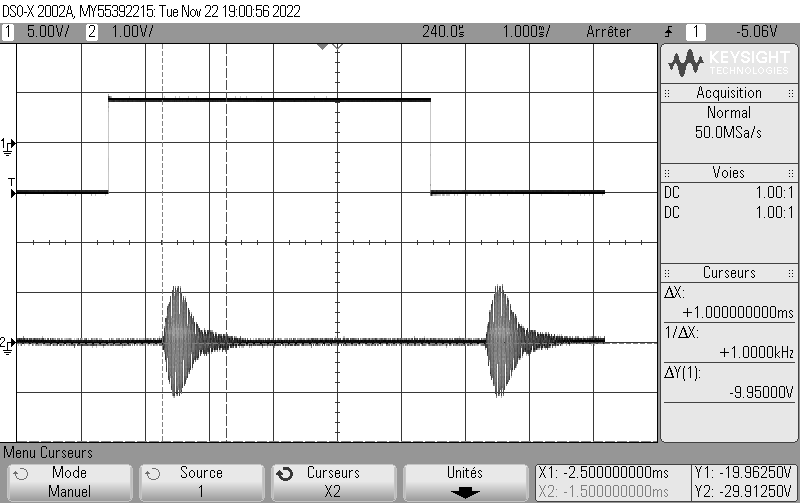
\includegraphics[width=0.4\textwidth]{figures/scope_2.png}
		\caption{Signal reçu après transmission d'un signal créneau.}
		\label{fig:cre-passe-bande}
	\end{figure}

	Ce signal est de la forme d'un \guillemotleft~paquet d'ondes.~\guillemotright\ Ainsi, on a l'approximation suivante : \[
		\mathrm{\Delta}f \simeq \frac{1}{\tau_\mathrm{c}}
	\] où $\tau_\mathrm{c}$\/ est la durée de cohérence.
	À l'oscilloscope, on mesure cette durée et on trouve $\tau_\mathrm{c} \simeq 1{,}0\: \mathrm{ms}$.
	On mesure ensuite la fréquence de résonance du signal : comme la fréquence de résonance est bien plus petite que celle du signal, la fréquence des harmoniques extraites sera proche de la fréquence de résonance recherchée. On mesure cette fréquence, comme montré dans la figure~\ref{fig:cre-passe-bande-zoom}. On trouve une fréquence de $f_\mathrm{r} \simeq 40{,}245\:\mathrm{kHz}$, ce qui correspond à la fréquence trouvée précédemment.

	\begin{figure}[H]
		\centering
		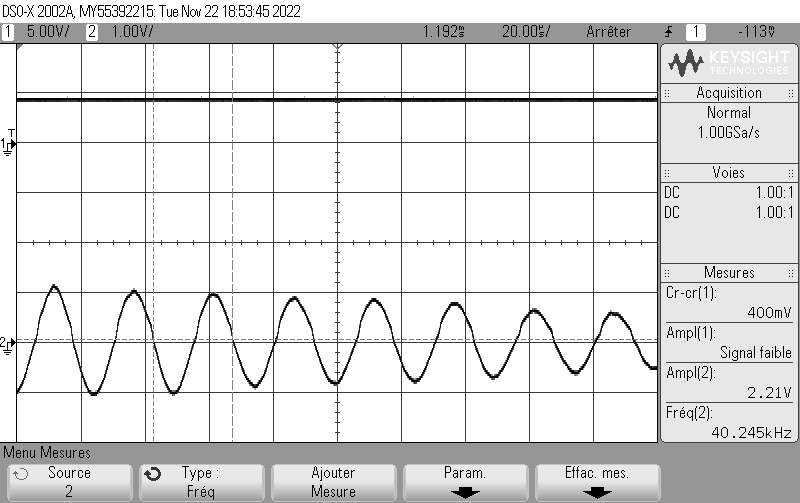
\includegraphics[width=0.4\textwidth]{figures/scope_1.png}
		\caption{Mesure d'une approximation de la fréquence de résonance.}
		\label{fig:cre-passe-bande-zoom}
	\end{figure}

	À l'aide de la formule du facteur de qualité du filtre passe-bande, et des mesures réalisées, on en déduit que \[
		{\color{cyan}Q \simeq \tau_\mathrm{c} \cdot f_{\mathrm{r}} \simeq 40},
	\] ce qui correspond approximativement à la valeur trouvée précédemment.
	En pratique, même si le facteur de qualité n'est qu'une approximation, cette méthode est plus simple à mettre en œuvre : un seul signal est généré et la fréquence ne varie pas, une seule acquisition suffit (contrairement à la méthode précédente).

	\section{Influence de l'angle émetteur-récepteur}
	L'objectif de cette partie du \textsc{tp} est la réalisation d'un \textit{diagramme de rayonnement} : un graphe polaire de l'amplitude en fonction de l'angle $\theta$\/ entre l'émetteur et le récepteur.
	Pour réaliser ce graphe, on fixe la distance émetteur-récepteur, et on tourne précisément l'émetteur d'un angle $\theta$.
	En pratique, on fixe l'émetteur sur un cavalier rotatif.
	Pour ces différentes valeurs de $\theta$, on mesure, à l'oscilloscope, l'amplitude du signal reçu. Au \textsc{gbf}, on génère à présent un signal sinusoïdal de fréquence $f$\/ proche de $f_\mathrm{r}$, pour avoir le plus de résolution dans la mesure de l'amplitude.

	\begin{figure}[H]
		\centering
		\begin{asy}
			import graph;

			real[] data = {
				9.6, 9.4, 9.3, 9, 8, 6.3, 4.3, 2.3,
				0.3, 1.3, 2, -1, 3, -1, 2.6, -1, 1.8,
				-1, 1
			};

			for(int i = 0; i <= 180; i += 10) {
				draw((0,0)--10dir(i), gray+dashed);
				if(i % 90 != 0)
					label("$" + string(90-i) + "^\circ$", 10.5 * dir(i));
			}

			for(int i = 1; i <= 10; ++i) {
				draw(arc((0,0), i * 1.0, 0, 180));
			}

			draw((-11,0)--(11,0), Arrow(TeXHead));
			draw((0,0)--(0,11), Arrow(TeXHead));

			pair[] points;

			for(int i = 0; i < data.length; ++i) {
				real angle = i * 5;
				real r = data[i];

				if(r < 0) continue;

				pair p1 = r * dir(angle + 90);
				points.push(p1);
			}

			for(int i = 0; i < points.length - 1; ++i) {
				pair p1 = points[i];
				pair p2 = points[i+1];
				draw(p1--p2, red);
				draw((-p1.x,p1.y)--(-p2.x,p2.y), red);
			}

			for(int i = 0; i < points.length; ++i) {
				pair p = points[i];
				dot(p, red);
				dot((-p.x, p.y), red);
			}

			size(16cm);
		\end{asy}
		\caption{\rlap{Diagramme de rayonnement de la chaîne}}
	\end{figure}

	Contrairement à ce que l'on peut penser, l'émetteur à ultra-sons n'émet pas uniquement devant lui. En effet, vers $45^\circ$, l'amplitude reçue est bien plus faible ; mais, avec des angles plus importants (comme $60^\circ$\/ ou $70^\circ$), l'amplitude transmise est bien plus importante.

	Nous n'avons mesurés qu'avec un angle $\theta$\/ positif, mais, il est possible que le système ne soit pas symétrique, et que le récepteur et/ou l'émetteur ait un défaut de symétrie.

	Nous n'avons pas eu le temps de finir la dernière partie du \textsc{tp} sur la vitesse de groupe et la vitesse de phase.

	\centerline{\pgfornament[width=3cm]{88}}

	Pour résumer, l'ensemble de la chaîne émission--transmission--réception ultra-sonore présente un caractère ``passe-bande.'' Cette particularité justifie l'observation de paquets d'ondes après la transmission d'un signal créneau. À partir de ces paquets d'ondes, on peut estimer la fréquence de résonance et le facteur de qualité du filtre passe-bande.
Au delà de la distance émetteur-récepteur, l'amplitude du signal dépend aussi de l'angle formé entre la direction d'observation et la normale à la surface d'émission. Elle est maximale pour un angle nul, négligeable pour un angle de $\pm 45^\circ$, et de nouveau présente pour des angles de $60$--$70^\circ$.

	\sign

	~

	\vspace{15cm}

	~
\end{document}
